% Figure from MATH 591 notes, section 70. Added, not from lecture (Lecture 25): flow boxes covering a compact manifold.
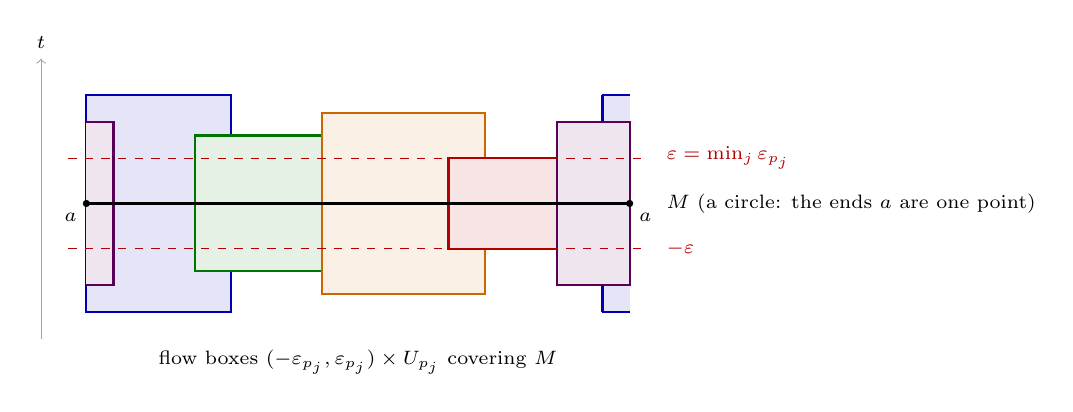
\begin{tikzpicture}[x=1.15cm, y=1.15cm]
\fill[blue!70!black!10] (0.00,-1.2) rectangle (1.60,1.2); \draw[blue!70!black, thick] (0.00,-1.2) rectangle (1.60,1.2);
\fill[blue!70!black!10] (5.70,-1.2) rectangle (6,1.2); \draw[blue!70!black, thick] (5.70,-1.2) -- (6,-1.2) (5.70,1.2) -- (6,1.2) (5.70,-1.2) -- (5.70,1.2);
\fill[green!45!black!10] (1.20,-0.75) rectangle (3.00,0.75); \draw[green!45!black, thick] (1.20,-0.75) rectangle (3.00,0.75);
\fill[orange!80!black!10] (2.60,-1.0) rectangle (4.40,1.0); \draw[orange!80!black, thick] (2.60,-1.0) rectangle (4.40,1.0);
\fill[red!70!black!10] (4.00,-0.5) rectangle (5.60,0.5); \draw[red!70!black, thick] (4.00,-0.5) rectangle (5.60,0.5);
\fill[violet!70!black!10] (5.20,-0.9) rectangle (6.00,0.9); \draw[violet!70!black, thick] (5.20,-0.9) rectangle (6.00,0.9);
\fill[violet!70!black!10] (0,-0.9) rectangle (0.30,0.9); \draw[violet!70!black, thick] (0,-0.9) -- (0.30,-0.9) -- (0.30,0.9) -- (0,0.9);
\draw[red!70!black, dashed] (-0.2,0.5) -- (6.2,0.5); \draw[red!70!black, dashed] (-0.2,-0.5) -- (6.2,-0.5);
\node[red!70!black, font=\scriptsize, anchor=west] at (6.3,0.5) {$\varepsilon = \min_j \varepsilon_{p_j}$};
\node[red!70!black, font=\scriptsize, anchor=west] at (6.3,-0.5) {$-\varepsilon$};
\draw[black, thick] (0,0) -- (6,0); \fill (0,0) circle (1.3pt); \fill (6,0) circle (1.3pt);
\node[font=\scriptsize, below left] at (0,0) {$a$}; \node[font=\scriptsize, below right] at (6,0) {$a$};
\node[font=\scriptsize, anchor=west] at (6.3,0) {$M$ (a circle: the ends $a$ are one point)};
\draw[->, gray!70] (-0.5,-1.5) -- (-0.5,1.6) node[above, font=\scriptsize, text=black] {$t$};
\node[font=\scriptsize, align=center] at (3,-1.75) {flow boxes $(-\varepsilon_{p_j}, \varepsilon_{p_j}) \times U_{p_j}$ covering $M$};
\end{tikzpicture}
